\section{Sécurité}
\subsection{Frontend}
\subsubsection{Routage}
\subsection{Backend}
\subsubsection{Routage API}
\subsubsection{Base de données}
\subsubsection{En-têtes HTTPS}

\subsection{Web Server}
\subsubsection{Configuration de base}
Lors de la location d'un VPS au près d'un fournisseur, il est essentiel de le configurer. Dans un premier temps, j'ai créer un utilisateur dédié pour mon application et supprimer l'utilisateur reçu lors de la location.
Par la suite, j'ai reconfigurer le service SSH afin de interdir la connexion par mot de passe, d'interdir la connexion en tant que root et d'autoriser la connexion par clé publique/privé.

De plus, afin de sécuriser le VPS contre les attaques par brute forces sur le port part défaut de SSH (port 22), j'ai reconfigurer celui-ci sur le port 3333.


\subsubsection{Firewall}
\subsubsection{Reverse-proxy}

\subsection{Autres}
\subsubsection{Libraries}

Un projet de cette envergure nécessite l'installation de plusieurs dépendances. Lorsque qu'une vulnerabilité a été découverte au niveau d'une des dépendances, il faut absolument réaliser une mise à jour dans les plus brefs délais.
C'est pourquoi l'utilisation d'un outil tel que \textbf{Dependabot} est nécessaire.

Dependabot est un outil intégré à github qui analyse de manière régulière les dépendances utilisées dans le projet afin de détecter d'éventuelles vulnérabilités. S'il en trouve une, cet outil envoie une alerte avec le niveau de danger qu'que la dépendance représente. Mais le plus intéressant, c'est qu'en plus des alertes, Dependabot crée une pull-request qu'il suffit d'accepter pour maintenir la dépendance à jour.



  \begin{figure}[H]
    \begin{minipage}[b]{0.5\linewidth}
    \centering
    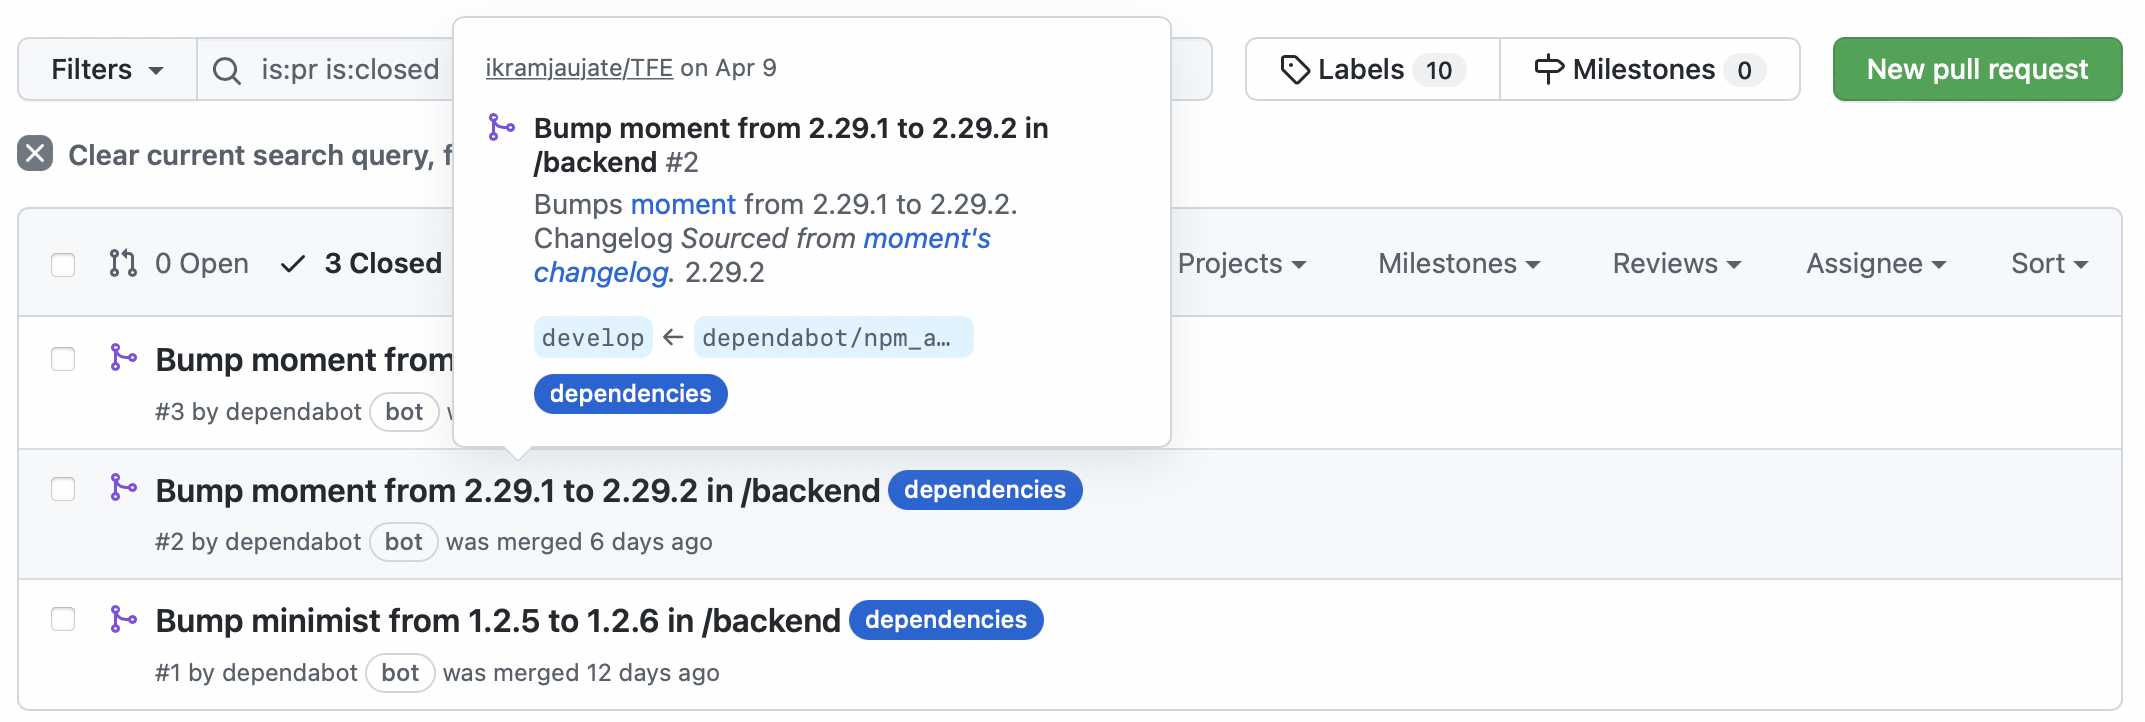
\includegraphics[width=1\linewidth]{img/depe.png}
    \caption{Pull-Request crée par Dependabot}
    \label{fig:figura1}
    \end{minipage}
    \hspace{0.3cm}
    \begin{minipage}[b]{0.5\linewidth}
    \centering
    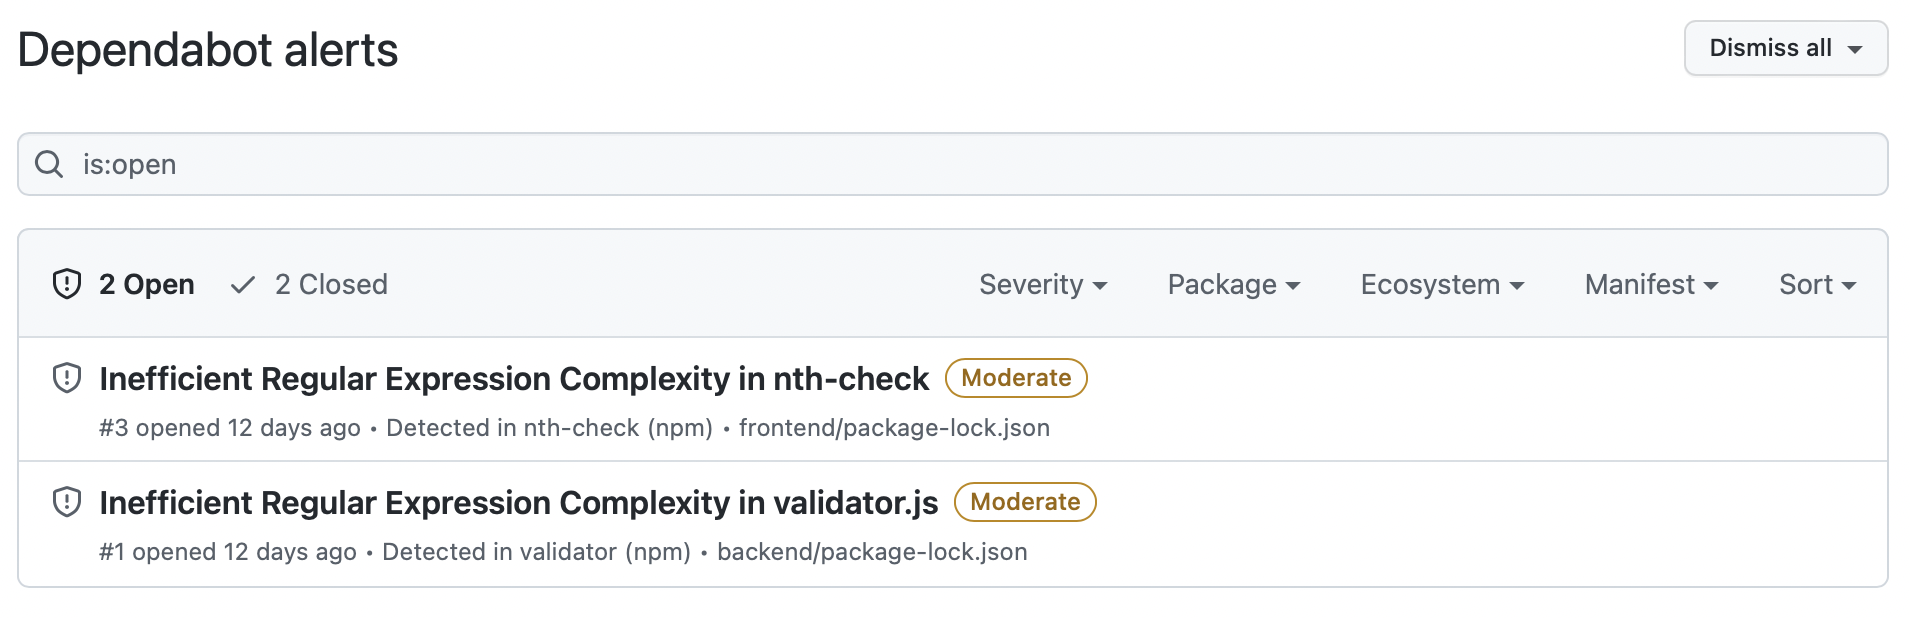
\includegraphics[width=1\linewidth]{img/alerts.png}
    \caption{Alertes générées par Dependabot}
    \label{fig:figura2}
    \end{minipage}
    \end{figure}




